%%%%%%%%%%%%%%%%%%%%%%%%%%%%%%%%%%%%%%%%%%%%%%%%%%%%%%%%%%%%%%%%%%%%%%%%%%%%%%%
%%%%%%%%%%%%%%%%%%%%%%%%%%%%%%%%%%%%%%%%%%%%%%%%%%%%%%%%%%%%%%%%%%%%%%%%%%%%%%%
%%%%%%%%%%%%%%%%%%%%%%%%%%%%%%%%%%%%%%%%%%%%%%%%%%%%%%%%%%%%%%%%%%%%%%%%%%%%%%%
\section{Implementation}
%
The SOSflow library and daemon codes are programmed in C99 and have
minimal external dependencies:
%
\begin{itemize}
    \item Message Passing Interface (MPI)
      %
    \item pthreads
      %
    \item SQLite
      %
\end{itemize}
%
SOSflow's core routines allow it to:
%
\begin{itemize}
      %
    \item Facilitate online capture of data from many sources.
      %
    \item Annotate the gathered data with context and meaning.
      %
    \item Store the captured data on-node in a way that can be
      searched with dynamic queries in real-time as well as being
      suitable for aggregation and long-term archival.
      %
\end{itemize}
%
%
SOSflow is divided into several components, central among them:
%
\begin{itemize}
      %
    \item \textbf{libsos} - Library of common routines for interacting with
      sosd daemons and SOS data structures.
      %
    \item \textbf{sosd\_listener} - Daemon process running on each node.
      %
    \item \textbf{sosd\_db} - Daemon process running on dedicated resources
      that stores data aggregated from one or more in situ daemons.
      %
    \item \textbf{sosa} - Analytics framework for online query of SOS data.
      %
\end{itemize}

\subsection{Architecture Overview} %------------------------------------------%
%%%%%
%\begin{figure}[h]
%  \centering
%  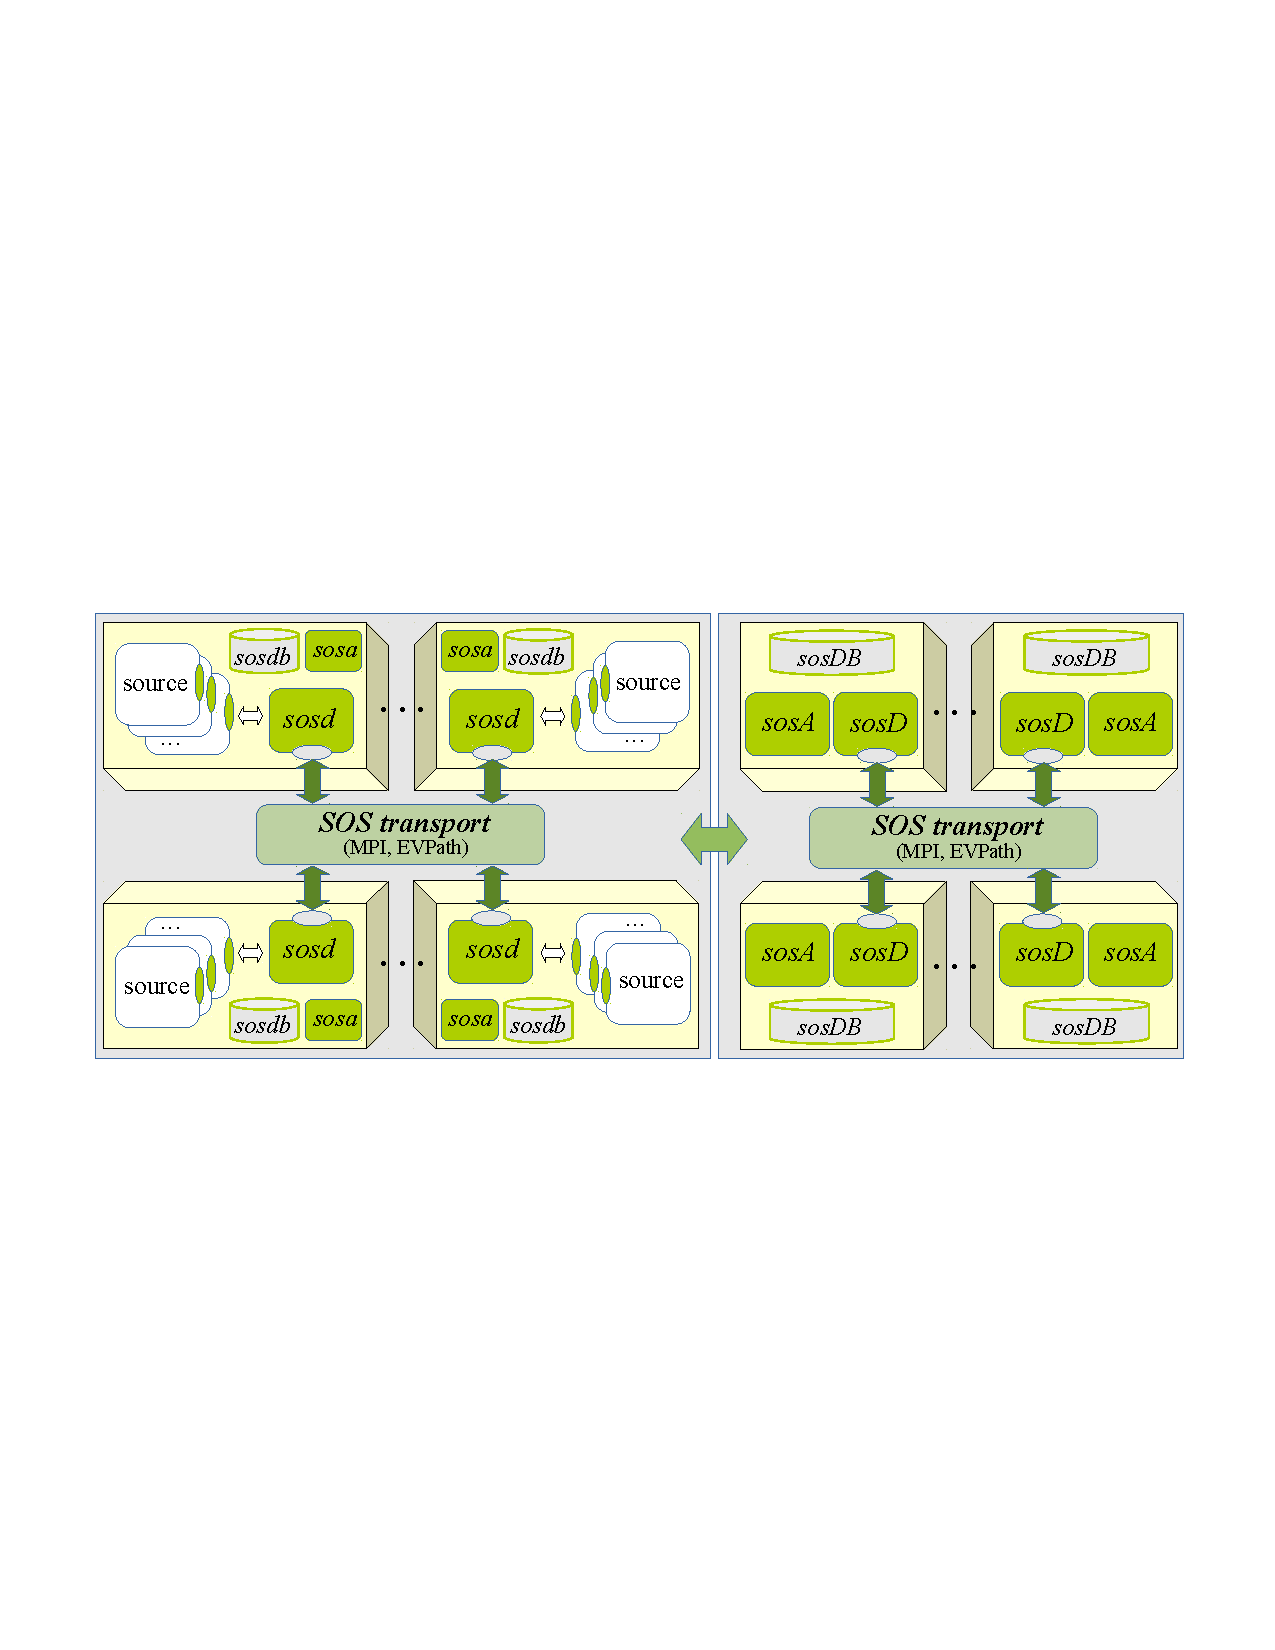
\includegraphics[width=\columnwidth]{images/sos.pdf}
%  \caption{SOSflow Internal Topology}
%  \label{fig_sos_topology}
%\end{figure}
%%%%%


%%%%%
%\begin{figure}[h]
%\centering
%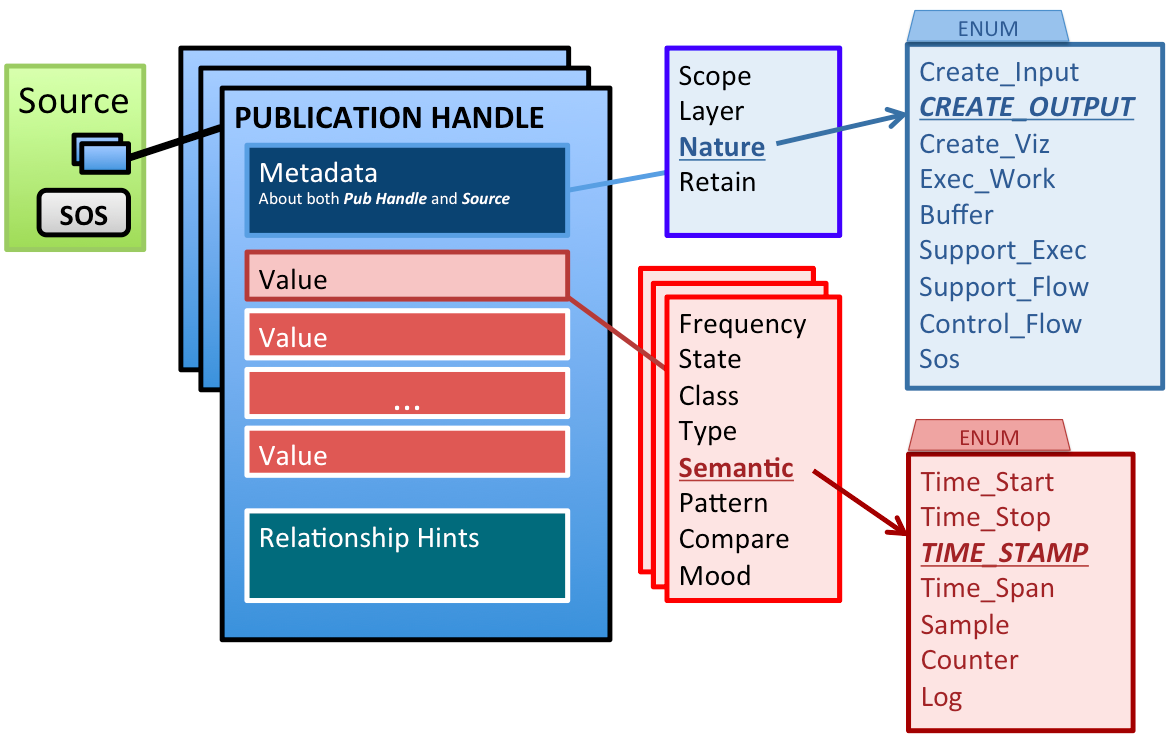
\includegraphics[width=\columnwidth]{images/pub_handle.png}
%\caption{Structure of an SOS Publication Handle}
%\label{fig_pub_handle}
%\end{figure}
%%%%%

%%%%%
Data in SOSflow is stored in a ``publication handle'' (pub) object.
%
This object organizes all of the application context information and
value-specific metadata, as well as managing the history of updates to
a value pending transmission to a sosd\_listener, called
\textit{value snapshots}.
%
Every value that is passed through the SOSflow API is preserved and
eventually stored in a searchable database, along with any updated
metadata such as its timestamp tuples.
%
%Multiple updates to the same value prior to a call to the publish API
%are no exception.
%
Prior value snapshots are queued and transmitted along
with the most recent update to that value.
%%%%%
%%%%%
\begin{figure}[h]
\centering
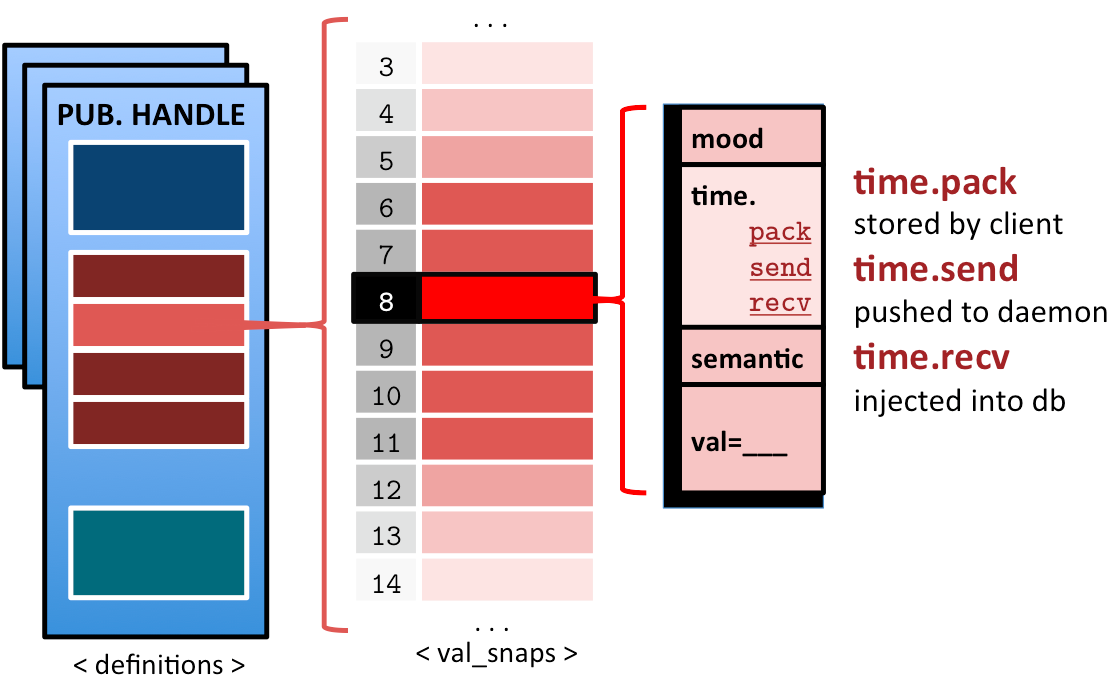
\includegraphics[width=\columnwidth]{images/val_snaps.png}
\caption{Complete History of Changing Values is Kept, Including Metadata}
\label{fig_val_snaps}
\end{figure}
%%%%%
%
\par
%
SOSflow utilizes different information transport methods
and communication patterns where appropriate \cite{aaziz2015push}.
%
Communication between client applications and their on-node daemon
takes place over a TCP socket connection.
%
%%%%%
\begin{figure}[h]
\centering
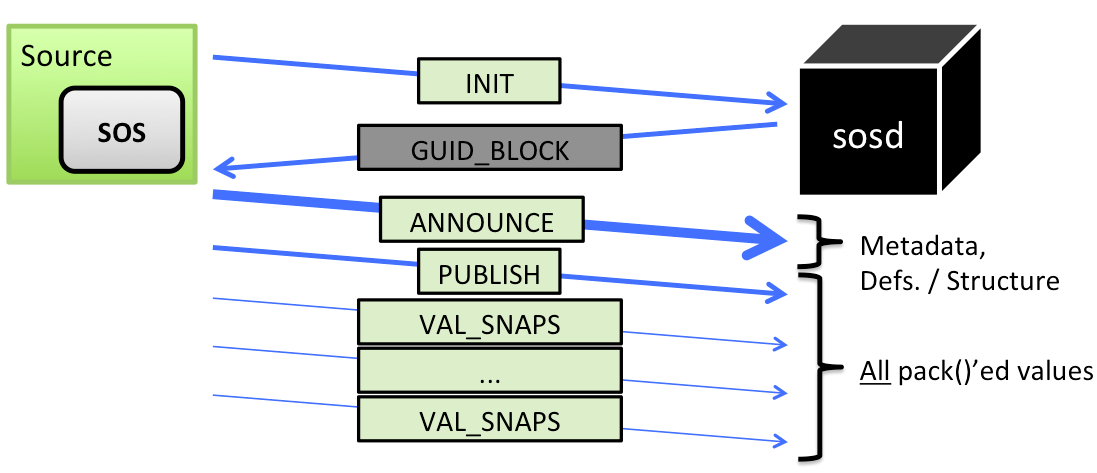
\includegraphics[width=\columnwidth]{images/sosd_protocol.png}
\caption{Client/Daemon Socket Communication Protocol}
\label{fig_sosd_protocol}
\end{figure}
%%%%%
%
Messages read from the socket are immediately placed in the daemon's
asynchronous queues to be processed by a worker thread.
%
The socket is then ready for the next queued message to
be received.
%
Messages are first enqueued for storage into an on-node database.
%
The same message is re-enqueued for transmission to an off-node data
aggregation target.
%
The SOSflow runtime uses MPI and the high-speed interconnect network
of the HPC machine when transmitting information off-node.
%%%%
%\begin{figure}[h]
%  \centering
%  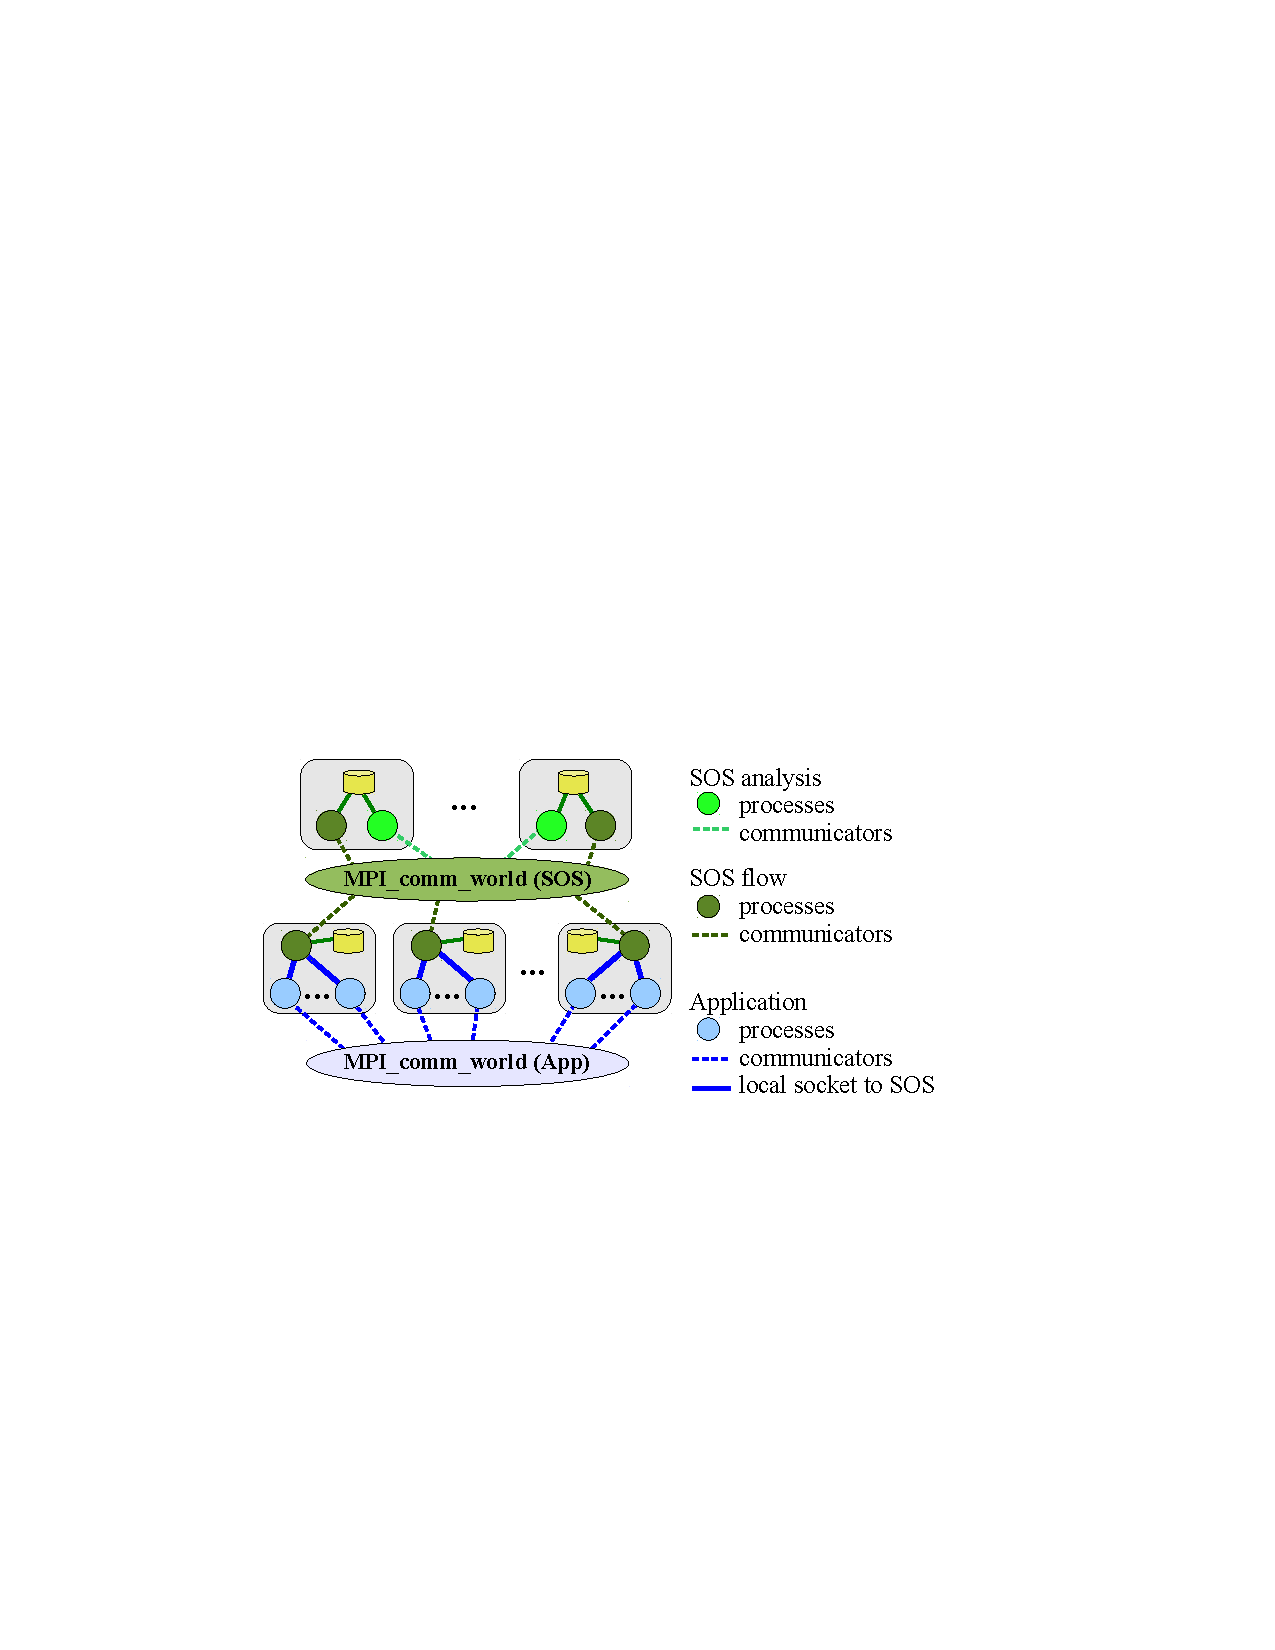
\includegraphics[width=\columnwidth]{images/sos-mpmd.pdf}
%  \caption{SOSflow Communicates w/MPI and Sockets}
%  \label{fig_sos_mpmd}
%\end{figure}
%%%%%
%
SOSflow does not participate in the MPI communicator[s] of the
applications that it is monitoring, so no special integration
programming is required of application developers who already use MPI
or sockets in their code.
%
\par
%
%
\subsection{Library: libsos} %------------------------------------------------%
%
Applications that make direct use of SOSflow through its API are called
\textit{clients}.
%
Clients must link in the libsos library which provides them with all of
the data structures and routines essential for interacting with
the SOSflow runtime platform.
%
The library routines are thread-safe, and no process-wide state is
maintained within the library, allowing application components to
interact with SOSflow independent of each other.
%
\par
%%
The primary interaction between a client and SOSflow is through the pub.
%
When a client initializes its SOSflow instance, it communicates with the
daemon and obtains a set of global unique ID (GUID) tags.
%
Clients pack values into a pub and they are automatically assigned a GUID.
%
When the client publishes that handle, all values are transmitted to
the SOSflow on-node daemon, including the complete history of each
value's updates from the last to the present publish call.
%
\par
%
All communication functions in the SOSflow client library are
handled transparently.
%
Users need only interact with a simple API to define and store values
that they can then publish to the daemon as appropriate.
%
The protocols and the codes of the client library are designed to be
fast and minimize resource usage, though they will buffer values for
the user if they choose to hold them and only transmit to the daemon
at intervals.
%
\par
%
Communications with the sosd\_listener are always initiated by the
clients, such as when they explicitly publish their pub.
%
SOSflow clients can voluntarily spawn a light-weight background thread
that periodically checks with their local daemon to see if any
feedback has been sent for them.
%
This loosely-coupled interactivity allows for run-time feedback to
happen independent of an application's schedule for transmitting its
information to SOSflow.
%
%

\subsection{Daemon: sosd\_listener} %-----------------------------------------%
The sosd daemon is itself an MPI application, and it is launched as a
background process in the user space at the start of a job script, before
the scientific workflow begins.
%
The daemons first go through a coordination phase where they each
participate in an MPI\_Allreduce() with all other daemon ranks in
order to share their role (DAEMON, DB, or ANALYTICS) and the name of
the host they are running on.
%
During the coordination phase, listener daemons select the sosd\_db
aggregate database that they will target for automatic asynchronous
transfer of the data they capture.
%
After initialization, SOSflow does not perform any further collective
communications.
%
%

\subsection{Database: sosd\_db} %---------------------------------------------%
%
The open-source SQLite database engine is used by sosd\_db for the on-node
database.
%
SQLite databases are persistent, lightweight, fast, and flexible, suitable to receive
streams of tuple data with very low overhead.
%
SOSflow provides a simple API for interacting with its database to streamline
access both on and off-node.
%
\par
%
At the time of this writing, SQLite technology is also used for the
aggregate databases, though work is ongoing to provide alternatives
for aggregation, starting with an interface to the Cassandra database.
%
%

\subsection{Analytics: sosa} %------------------------------------------------%
%
SOSflow analytics modules are independent programs that are launched
and operate alongside the SOSflow run-time.
%
The primary role of the analytics modules is to query the database and
produce functional output such as real-time visualizations of
performance metrics, feedback to facilitate optimizations, or global
resource bound calculation and policy enforcement.
%
%(Figure~\ref{example_query})
%
%\begin{figure}[h]
%\centering
%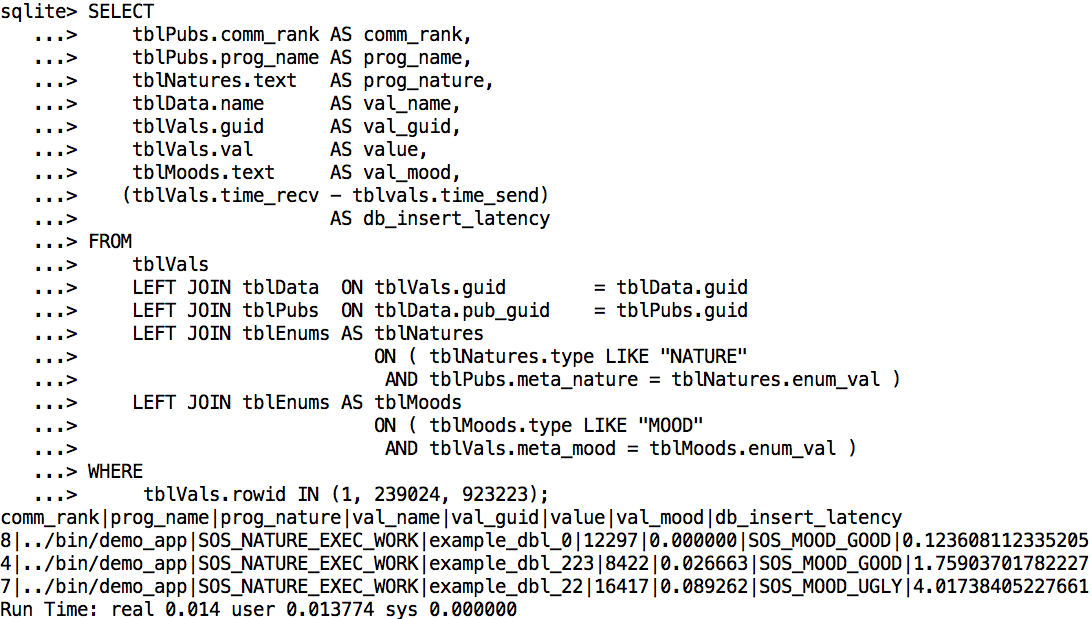
\includegraphics[width=\columnwidth]{images/query_example.png}
%\caption{Example of Querying the SOSflow Database}
%\label{example_query}
%\end{figure}
%
The modules can be deployed in a distributed fashion to run on the nodes
where the applications are executing, or they can be deployed on dedicated
resources and coupled with the aggregate databases for fast queries
of the global state.
%
Analytics modules have the ability to make use of the high-speed
interconnect of the HPC machine in order to share data amongst themselves.
%
\par
%
SOSflow provides an API for client applications to register
a callback function with a named trigger handle.
%
Those triggers can be fired off by analytics modules, and arbitrary
data structures can be passed to the triggered functions.
%
Triggers may be fired for a specific single process on one node,
or for an entire node, or an entire scientific workflow.
%
This capability facilitates the use of SOSflow as a general-purpose observation,
introspection, feedback, and control platform.
%%%%%
%%%
%%%  EOF
%%%
